\documentclass[]{article}

\usepackage[utf8]{inputenc}
\usepackage[T1]{fontenc}
\usepackage{lmodern}
\usepackage{textgreek}
\usepackage{newunicodechar}
\newunicodechar{⁰}{\ensuremath{^0}}
\newunicodechar{²}{\ensuremath{^2}}
\newunicodechar{³}{\ensuremath{^3}}
\newunicodechar{₁}{\ensuremath{_1}}
\newunicodechar{₂}{\ensuremath{_2}}
\newunicodechar{₃}{\ensuremath{_3}}
\newunicodechar{×}{\ensuremath{\times}}
\newunicodechar{∇}{\ensuremath{\nabla}}
\newunicodechar{≈}{\ensuremath{\approx}}
\newunicodechar{≡}{\ensuremath{\equiv}}
\newunicodechar{≤}{\ensuremath{\leq}}
\newunicodechar{≥}{\ensuremath{\geq}}
\newunicodechar{→}{\ensuremath{\rightarrow}}
\newunicodechar{←}{\ensuremath{\leftarrow}}
\newunicodechar{↑}{\ensuremath{\uparrow}}
\newunicodechar{↓}{\ensuremath{\downarrow}}
\newunicodechar{↔}{\ensuremath{\leftrightarrow}}
\newunicodechar{—}{\textemdash}
\newunicodechar{–}{\textendash}
\newunicodechar{−}{\ensuremath{-}}
\newunicodechar{√}{\ensuremath{\surd}}
\newunicodechar{∼}{\ensuremath{\sim}}
\newunicodechar{≲}{\ensuremath{\lesssim}}
\newunicodechar{≳}{\ensuremath{\gtrsim}}
\newunicodechar{⟨}{\ensuremath{\langle}}
\newunicodechar{⟩}{\ensuremath{\rangle}}
\newunicodechar{₀}{\ensuremath{_0}}
\newunicodechar{₄}{\ensuremath{_4}}
\newunicodechar{₅}{\ensuremath{_5}}
\newunicodechar{₆}{\ensuremath{_6}}
\newunicodechar{₇}{\ensuremath{_7}}
\newunicodechar{₈}{\ensuremath{_8}}
\newunicodechar{₉}{\ensuremath{_9}}
\newunicodechar{⁴}{\ensuremath{^4}}
\newunicodechar{α}{\ensuremath{\alpha}}
\newunicodechar{β}{\ensuremath{\beta}}
\newunicodechar{γ}{\ensuremath{\gamma}}
\newunicodechar{δ}{\ensuremath{\delta}}
\newunicodechar{ε}{\ensuremath{\epsilon}}
\newunicodechar{θ}{\ensuremath{\theta}}
\newunicodechar{λ}{\ensuremath{\lambda}}
\newunicodechar{μ}{\ensuremath{\mu}}
\newunicodechar{ν}{\ensuremath{\nu}}
\newunicodechar{ξ}{\ensuremath{\xi}}
\newunicodechar{π}{\ensuremath{\pi}}
\newunicodechar{ρ}{\ensuremath{\rho}}
\newunicodechar{σ}{\ensuremath{\sigma}}
\newunicodechar{τ}{\ensuremath{\tau}}
\newunicodechar{φ}{\ensuremath{\phi}}
\newunicodechar{ϕ}{\ensuremath{\phi}}
\newunicodechar{χ}{\ensuremath{\chi}}
\newunicodechar{ψ}{\ensuremath{\psi}}
\newunicodechar{ω}{\ensuremath{\omega}}
\newunicodechar{Δ}{\ensuremath{\Delta}}
\newunicodechar{Λ}{\ensuremath{\Lambda}}
\newunicodechar{Σ}{\ensuremath{\Sigma}}
\newunicodechar{Φ}{\ensuremath{\Phi}}
\newunicodechar{Ω}{\ensuremath{\Omega}}
\newunicodechar{“}{``}
\newunicodechar{”}{''}
\newunicodechar{‘}{`}
\newunicodechar{’}{'}
\usepackage{amsmath}
\usepackage{amssymb}
\usepackage{multirow}
\usepackage{natbib}
\usepackage{graphicx}
\usepackage{tabularx}
\usepackage{adjustbox}
\usepackage{listings}
\usepackage{hyperref}
\usepackage{xcolor}
\lstset{
  basicstyle=\ttfamily\footnotesize,
  backgroundcolor=\color{black!4},
  frame=none,
  breaklines=true,
  breakatwhitespace=true,
  showstringspaces=false,
  columns=fullflexible,
  xleftmargin=1em,
  xrightmargin=1em,
  aboveskip=0.6em,
  belowskip=0.6em,
  keywordstyle=\color{blue!60!black},
  commentstyle=\itshape\color{black!60},
  stringstyle=\color{green!50!black},
}
\usepackage[margin=1in]{geometry}


\begin{document}

\title{Decoupling Non-Additive Energetics via Graph-Latent Residual Decomposition}

\author{Denario}
\date{Anthropic, Gemini \& OpenAI servers. Planet Earth.}

\maketitle
\begin{abstract}
Classical group-contribution methods effectively capture the extensive scaling of molecular internal energy but inherently fail to account for non-additive electronic effects arising from complex topological features. To isolate and quantify these non-linear contributions, we propose a residual decomposition approach applied to the QM9 dataset. We first train a Ridge regression baseline on heavy atom and functional group counts to decouple the extensive energetic scaling. Subsequently, we employ a Graph Neural Network (GNN) to predict the standardized residuals of this additive baseline, utilizing Integrated Gradients and latent space dimensionality reduction to interpret the learned representations. The GNN successfully captures the topological variance missed by classical models, achieving a test $R^2$ of 0.9985 on the residuals and substantially outperforming a descriptor-based Random Forest baseline. Analysis of the GNN's 128-dimensional latent space reveals intrinsic correlations with fundamental intensive properties, such as the HOMO-LUMO gap and HOMO energy, despite the absence of direct supervision on these targets. Furthermore, structural motif attribution and statistical validation confirm that features such as aromaticity, nitrogen integration, and fluorine incorporation significantly drive these non-additive deviations, corresponding directly to compressed HOMO-LUMO gaps and shifted dipole moments. This framework rigorously separates extensive scaling from underlying non-linear electronic physics, demonstrating that graph-based message passing can effectively map specific structural motifs to their quantum-mechanical deviations from classical additivity.
\end{abstract}








\section{Introduction}
\label{sec:introduction}
Predicting the thermodynamic and quantum-mechanical properties of molecules is a central challenge in computational chemistry. For extensive properties such as the internal energy at 0 K ($U_0$), classical group-contribution methods have long provided a robust baseline. These models operate on the principle of additivity, effectively capturing the extensive scaling of molecular energy by summing the independent contributions of constituent atoms, bonds, and functional groups. However, while additive models excel at capturing size-dependent scaling, they inherently fail to account for non-additive electronic effects. Phenomena such as extended $\pi$-conjugation, aromaticity, and complex heteroatom interactions depend on the global topological structure of the molecule rather than mere constituent counts. Consequently, classical methods leave a residual variance that represents the underlying non-linear quantum-mechanical physics.To isolate and quantify these non-linear contributions, we propose a graph-latent residual decomposition framework, applied to the QM9 dataset \citep{fu2025benchmarkquantumchemistryrelaxations}. Our approach rigorously separates extensive scaling from non-additive electronic physics without requiring the generation of 3D atomic coordinates. We first decouple the extensive energetic scaling by training a Ridge regression baseline on heavy atom and functional group counts. The residuals of this additive model represent the purely non-additive energetic deviations. Subsequently, we employ a Graph Neural Network (GNN) to predict these standardized residuals \citep{schütt2016quantumchemicalinsightsdeeptensor,xiang2025edbenchlargescaleelectrondensity}. By operating directly on the molecular graph via message passing, the GNN is uniquely positioned to capture the long-range topological features and structural nuances that linear models and standard descriptor-based algorithms miss \citep{schütt2016quantumchemicalinsightsdeeptensor,esders2024analyzingatomicinteractionsmolecules,xiang2025edbenchlargescaleelectrondensity}.Beyond achieving high predictive accuracy, a primary objective of this work is to interpret the learned non-additive representations and connect them to established chemical theory \citep{wang2023graphneuralnetworksmolecules,liu2026latentflowvisualanalyticslatent,han2026multimodalmolecularrepresentationlearning}. To this end, we extract the 128-dimensional latent space from the GNN to investigate whether the network intrinsically learns fundamental intensive properties—such as the HOMO-LUMO gap, HOMO energy, and dipole moment ($\mu$)—despite receiving no direct supervision on these targets \citep{choi2022scalabletraininggraphconvolutional,liu2026enhancingmolecularpropertypredictions,chakraborty2026duallevelatomiccoordinationgeometry}. Furthermore, we apply Integrated Gradients to the trained network to map the predicted energetic deviations back to specific molecular subgraphs, enabling a quantitative assessment of which structural motifs exert the greatest influence on energetic stability.In this paper, we demonstrate that the GNN successfully captures the topological variance missed by classical models, substantially outperforming a descriptor-based Random Forest baseline. \citep{shui2020heterogeneousmoleculargraphneural,liu2021fastquantumpropertyprediction,rittig2022graphneuralnetworksprediction} Analysis of the latent space reveals strong, unsupervised correlations with fundamental electronic descriptors. \citep{lu2019molecularpropertypredictionmultilevel,liu2021fastquantumpropertyprediction,arjonamedina2024analysisatomlevelpretrainingquantum} Finally, through structural motif attribution and statistical validation, we confirm that specific features—namely aromatic rings and the integration of nitrogen and fluorine—significantly drive these non-additive deviations. \citep{shui2020heterogeneousmoleculargraphneural,wang2022motifbasedgraphrepresentationlearning,yu2025magemodellevelgraphneural} These motifs correspond directly to physically observable phenomena, such as compressed HOMO-LUMO gaps and shifted dipole moments, validating that our residual decomposition framework effectively maps specific structural motifs to their quantum-mechanical deviations from classical additivity. \citep{lu2019molecularpropertypredictionmultilevel,shui2020heterogeneousmoleculargraphneural,liu2021fastquantumpropertyprediction}

\section{Methods}
\label{sec:methods}
\subsection{Data preprocessing and quality control}The QM9 dataset was utilized to investigate the non-additive electronic contributions to molecular internal energy at 0 K ($U_0$). Molecular structures were parsed from SMILES strings using the RDKit library. During initial quality control, 83 duplicated SMILES representations were identified; to ensure consistent labeling and prevent training instability, the target property values for these duplicates were averaged. To rigorously evaluate model generalization and prevent data leakage, the dataset was partitioned into training (80\%), validation (10\%), and test (10\%) sets using a molecule-aware splitting strategy. This ensured that all instances of identical SMILES strings, if any remained after deduplication, resided within the same partition. For each molecule, explicit size-normalization features, including heavy atom counts and hydrogen counts, were calculated alongside counts of specific bond types and functional groups to serve as inputs for the classical additive baseline.\subsection{Baseline additive model construction}To decouple the extensive scaling inherent to the dataset from the underlying non-linear electronic physics, a Group Contribution Method (GCM) baseline was constructed using Ridge regression. The baseline model was trained exclusively on the training set to predict $U_0$ using the number of heavy atoms and the counts of various bond types and functional groups as independent variables. By modeling the purely additive components of the internal energy, the Ridge regression isolates the non-additive energetic deviations as residuals. For each molecule $i$, the residual $r_i$ was calculated as the difference between the actual internal energy and the baseline prediction:\begin{equation}    r_i = U_{0,i} - \hat{U}_{0,i}^{\text{Ridge}}\end{equation}To ensure stable gradient dynamics during the subsequent neural network training, these residuals were standardized using z-score normalization based on the training set mean ($\mu_r$) and standard deviation ($\sigma_r$):\begin{equation}    z_i = \frac{r_i - \mu_r}{\sigma_r} \citep{yun2024znormzscoregradientnormalization}\end{equation}These standardized residuals ($z_i$) served as the target variable for the non-linear models.\subsection{Graph neural network architecture and training}To capture the topological nuances and long-range electronic effects missed by the additive baseline, a Graph Neural Network (GNN) was designed to predict the standardized residuals \citep{gilmer2017neuralmessagepassingquantum,ma2020multiviewgraphneuralnetworks}. The molecular graphs were constructed with node features encoding atomic number, hybridization state, and atomic degree, while edge features encoded bond type and aromaticity \citep{ma2020multiviewgraphneuralnetworks,nguyen2026mmgnnmultilevelmulticolorgraph}.The network architecture employed message-passing layers to propagate local structural information across the molecular graph. \citep{gilmer2017neuralmessagepassingquantum,berry2025surveygraphneuralnetworks} To effectively aggregate global electronic effects, such as extended $\pi$-conjugation pathways, a Global Attention Pooling layer was incorporated. \citep{jo2021flexibledualbranchedmessagepassing,pescia2023messagepassingneuralquantumstates} The pooled graph-level representation was then passed through a multi-layer perceptron terminating in a linear output layer (without an activation function) to accommodate the unbounded continuous range of the standardized residuals. \citep{gilmer2017neuralmessagepassingquantum,liu2026localglobalmultimodalcontrastivelearning}The GNN was trained to minimize the Mean Squared Error (MSE) loss between the predicted and actual standardized residuals. Training was regulated using an early stopping criterion monitored on the validation loss to prevent overfitting. To benchmark the efficacy of the graph-based message passing, a Random Forest regressor was also trained on the same RDKit-derived descriptors used for the Ridge baseline. Comparing the GNN against this non-linear descriptor-based baseline isolates the performance gain attributable specifically to the explicit modeling of molecular topology.\subsection{Latent space extraction and analysis}To interpret the learned representations of non-additivity, the 128-dimensional latent vectors were extracted from the penultimate layer of the trained GNN for all molecules in the test set. This latent space was analyzed to determine whether the network intrinsically learned fundamental intensive properties without direct supervision.Dimensionality reduction was performed using t-Distributed Stochastic Neighbor Embedding (t-SNE) to visualize the embedding landscape and identify structural clustering . Both the raw 128-dimensional latent features and the reduced t-SNE components were statistically correlated (using Pearson $r$ and Spearman $\rho$ coefficients) with known intensive electronic properties provided in the QM9 dataset, specifically the HOMO-LUMO gap, HOMO energy, LUMO energy, and dipole moment ($\mu$) .\subsection{Structural motif attribution and statistical validation}To map the predicted non-additive energetics back to specific chemical features, the Integrated Gradients (IG) attribution method was applied to the trained GNN \citep{ji2026molledgeradditivegraphneural}. The baseline input for the IG algorithm was defined as a "null" graph, where all node and edge features were zeroed out. To ensure that the attribution scores were comparable across molecules of varying sizes, the raw IG scores were normalized by the total number of atoms in the molecule.Molecules were subsequently partitioned into groups based on the presence of high-influence topological features identified by the network, such as aromatic rings and the integration of specific heteroatoms (nitrogen, oxygen, and fluorine) \citep{esders2024analyzingatomicinteractionsmolecules,polat2025understandingcapabilitiesmoleculargraph}. To validate the physical relevance of these GNN-identified motifs, statistical tests were conducted to compare the distributions of intensive properties (HOMO-LUMO gap and dipole moment) between molecules containing these motifs and those without \citep{gilmer2017neuralmessagepassingquantum,choi2022scalabletraininggraphconvolutional}. Depending on the distribution of the data, Analysis of Variance (ANOVA) or non-parametric Kruskal-Wallis tests were employed to determine statistical significance, while Cohen's $d$ was calculated to quantify the effect size of each structural motif on the electronic properties.

\section{Results}
\label{sec:results}
\subsection{Extensivity decoupling and baseline performance}To isolate the non-additive electronic contributions to the internal energy ($U_0$), the extensive scaling inherent to the QM9 dataset was first decoupled using a classical group-contribution approach. The Ridge regression baseline, which predicted $U_0$ directly from heavy atom and functional group counts, yielded a test $R^2$ of 0.9850 and a test Mean Squared Error (MSE) of 23.6894. This confirms that while classical additivity captures the bulk of the extensive scaling, a meaningful residual variance remains, representing the purely non-additive energetics.To evaluate how well graph-based topological models capture this non-additivity compared to non-linear descriptor-based models, a Random Forest (RF) and a Graph Neural Network (GNN) were trained to predict the standardized residuals of the Ridge baseline. The Random Forest achieved a test $R^2$ of 0.9779 and a test MSE of 0.0209. In contrast, the GNN substantially outperformed the descriptor-based baseline, achieving a test $R^2$ of 0.9985 and a test MSE of 0.0014. By successfully modeling these deviations, the GNN demonstrates that explicit message passing over the molecular graph is highly effective at capturing the non-linear electronic physics that classical additivity models miss \citep{gilmer2017neuralmessagepassingquantum,rittig2022graphneuralnetworksprediction,panapitiya2025fragnetgraphneuralnetwork}. The relationship between these predicted non-additive residuals and fundamental intensive properties, such as the HOMO-LUMO gap and dipole moment, reveals that the modeled deviations are intrinsically linked to underlying quantum-mechanical phenomena rather than extensive scaling (Figure \ref{fig:image0}) \citep{gilmer2017neuralmessagepassingquantum,zhao2023molecularpropertypredictionbased}.\begin{figure}[!tbp]    \centering    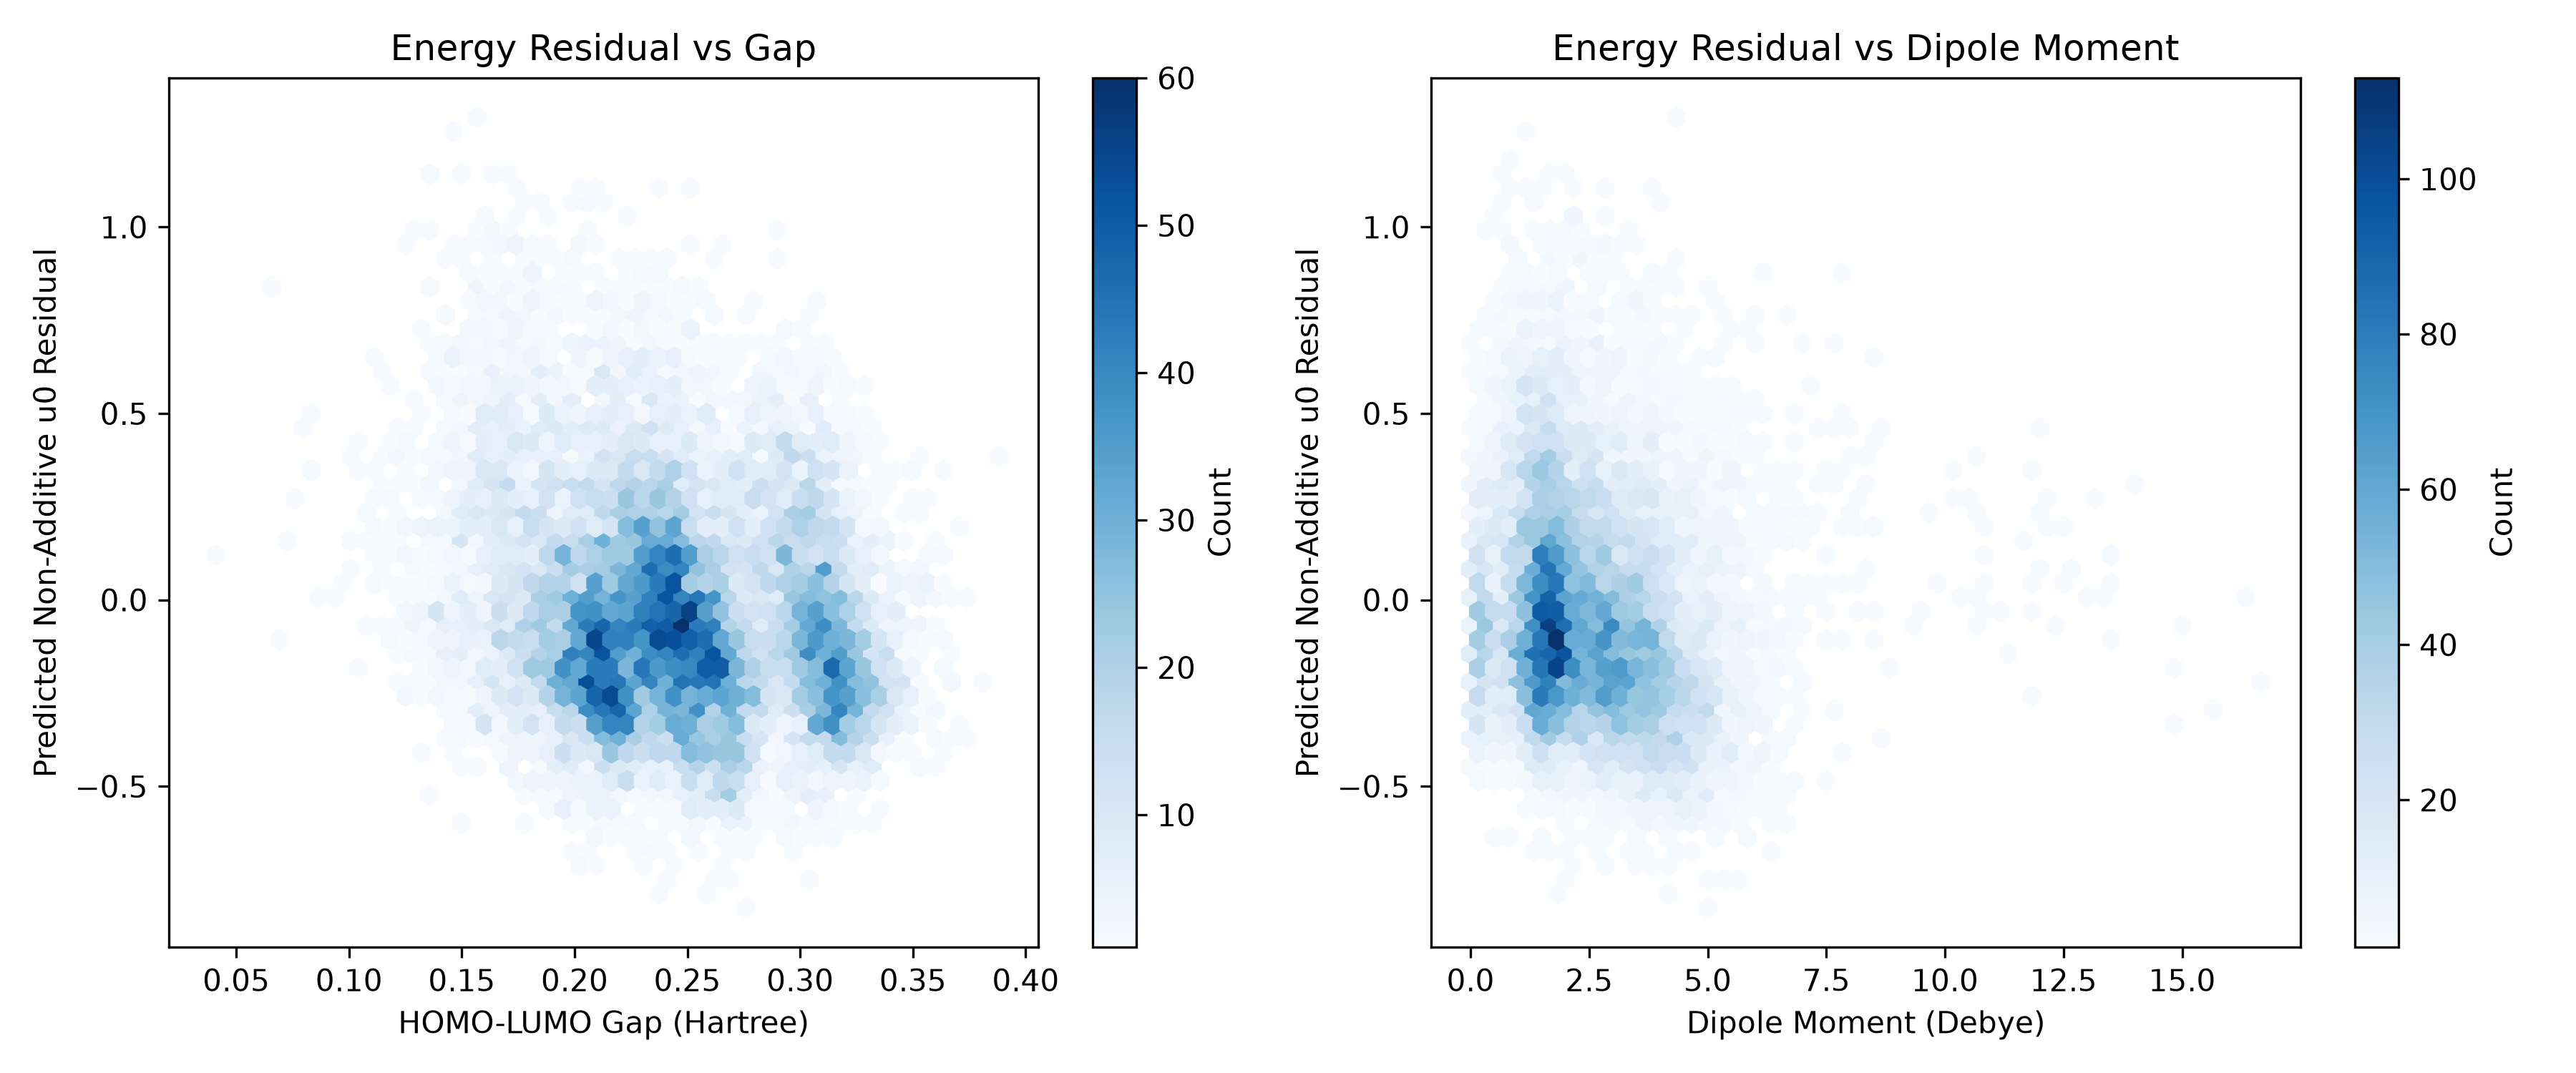
\includegraphics[width=0.99\textwidth]{../input_files/plots/residual_gap_corr.png}    \caption{Hexbin scatter plots illustrating the relationship between the predicted non-additive internal energy ($U_0$) residuals and fundamental intensive electronic properties: the HOMO-LUMO gap (left) and the dipole moment (right). The residuals represent energetic deviations from a classical additive baseline model. By mapping these predicted non-additive contributions against the gap and dipole moment—properties shown to be significantly driven by structural motifs such as extended $\pi$-conjugation and heteroatom electronegativity—the distributions reveal how non-linear electronic physics are captured by the Graph Neural Network. The observed clustering demonstrates that the modeled deviations from classical additivity are intrinsically linked to underlying quantum-mechanical phenomena rather than extensive scaling.}    \label{fig:image0}\end{figure}\subsection{Latent space and intensive property correlation}To interpret the learned representations of non-additivity, the 128-dimensional latent vectors were extracted from the penultimate layer of the trained GNN for the 13,381 molecules in the test set  \citep{rittig2022graphneuralnetworksprediction,wang2023graphneuralnetworksmolecules,xing2025learningcontinuoussolventeffects}. The extracted latent space exhibits a mean of $-0.2883$ and a standard deviation of $2.7265$.Analysis of this latent space confirms that the network intrinsically learned underlying electronic structures without direct supervision on these targets \citep{ye2019symmetricalgraphneuralnetwork,atlas2026latentspacedesigninteratomic}. Individual latent dimensions highly correlate with the modeled non-additive residual; for instance, latent dimension 24 correlates with the residual at a Pearson $r = -0.8520$, and dimension 102 at $r = 0.8274$ \citep{wu2019comprehensivesurveygraphneural}. Furthermore, these dimensions capture physical intensive properties: latent dimension 83 correlates with the HOMO-LUMO gap at $r = 0.5207$, and dimension 50 correlates with the HOMO energy at $r = 0.3756$ \citep{kosasih2021graphneuralnetworkensembles,schiff2022augmentingmoleculardeepgenerative,han2026multimodalmolecularrepresentationlearning}.Projecting this latent space into two dimensions using t-Distributed Stochastic Neighbor Embedding (t-SNE) further illustrates a structured embedding landscape (Figure \ref{fig:image2}) \citep{liu2021fastquantumpropertyprediction,choi2022scalabletraininggraphconvolutional}. The first principal dimension of the projection correlates with the HOMO-LUMO gap (Pearson $r = -0.3635$, Spearman $\rho = -0.3414$) and HOMO energy ($r = 0.3068$) \citep{gilmer2017neuralmessagepassingquantum,zhang2021litegemlitegeometryenhanced}. The second dimension strongly orders the target non-additive residual (Spearman $\rho = 0.7871$, Pearson $r = 0.4611$). These distinct property gradients confirm that the GNN effectively models the non-linear electronic physics missed by classical additivity models \citep{ye2019symmetricalgraphneuralnetwork,kosasih2021graphneuralnetworkensembles}.\begin{figure}[!tbp]    \centering    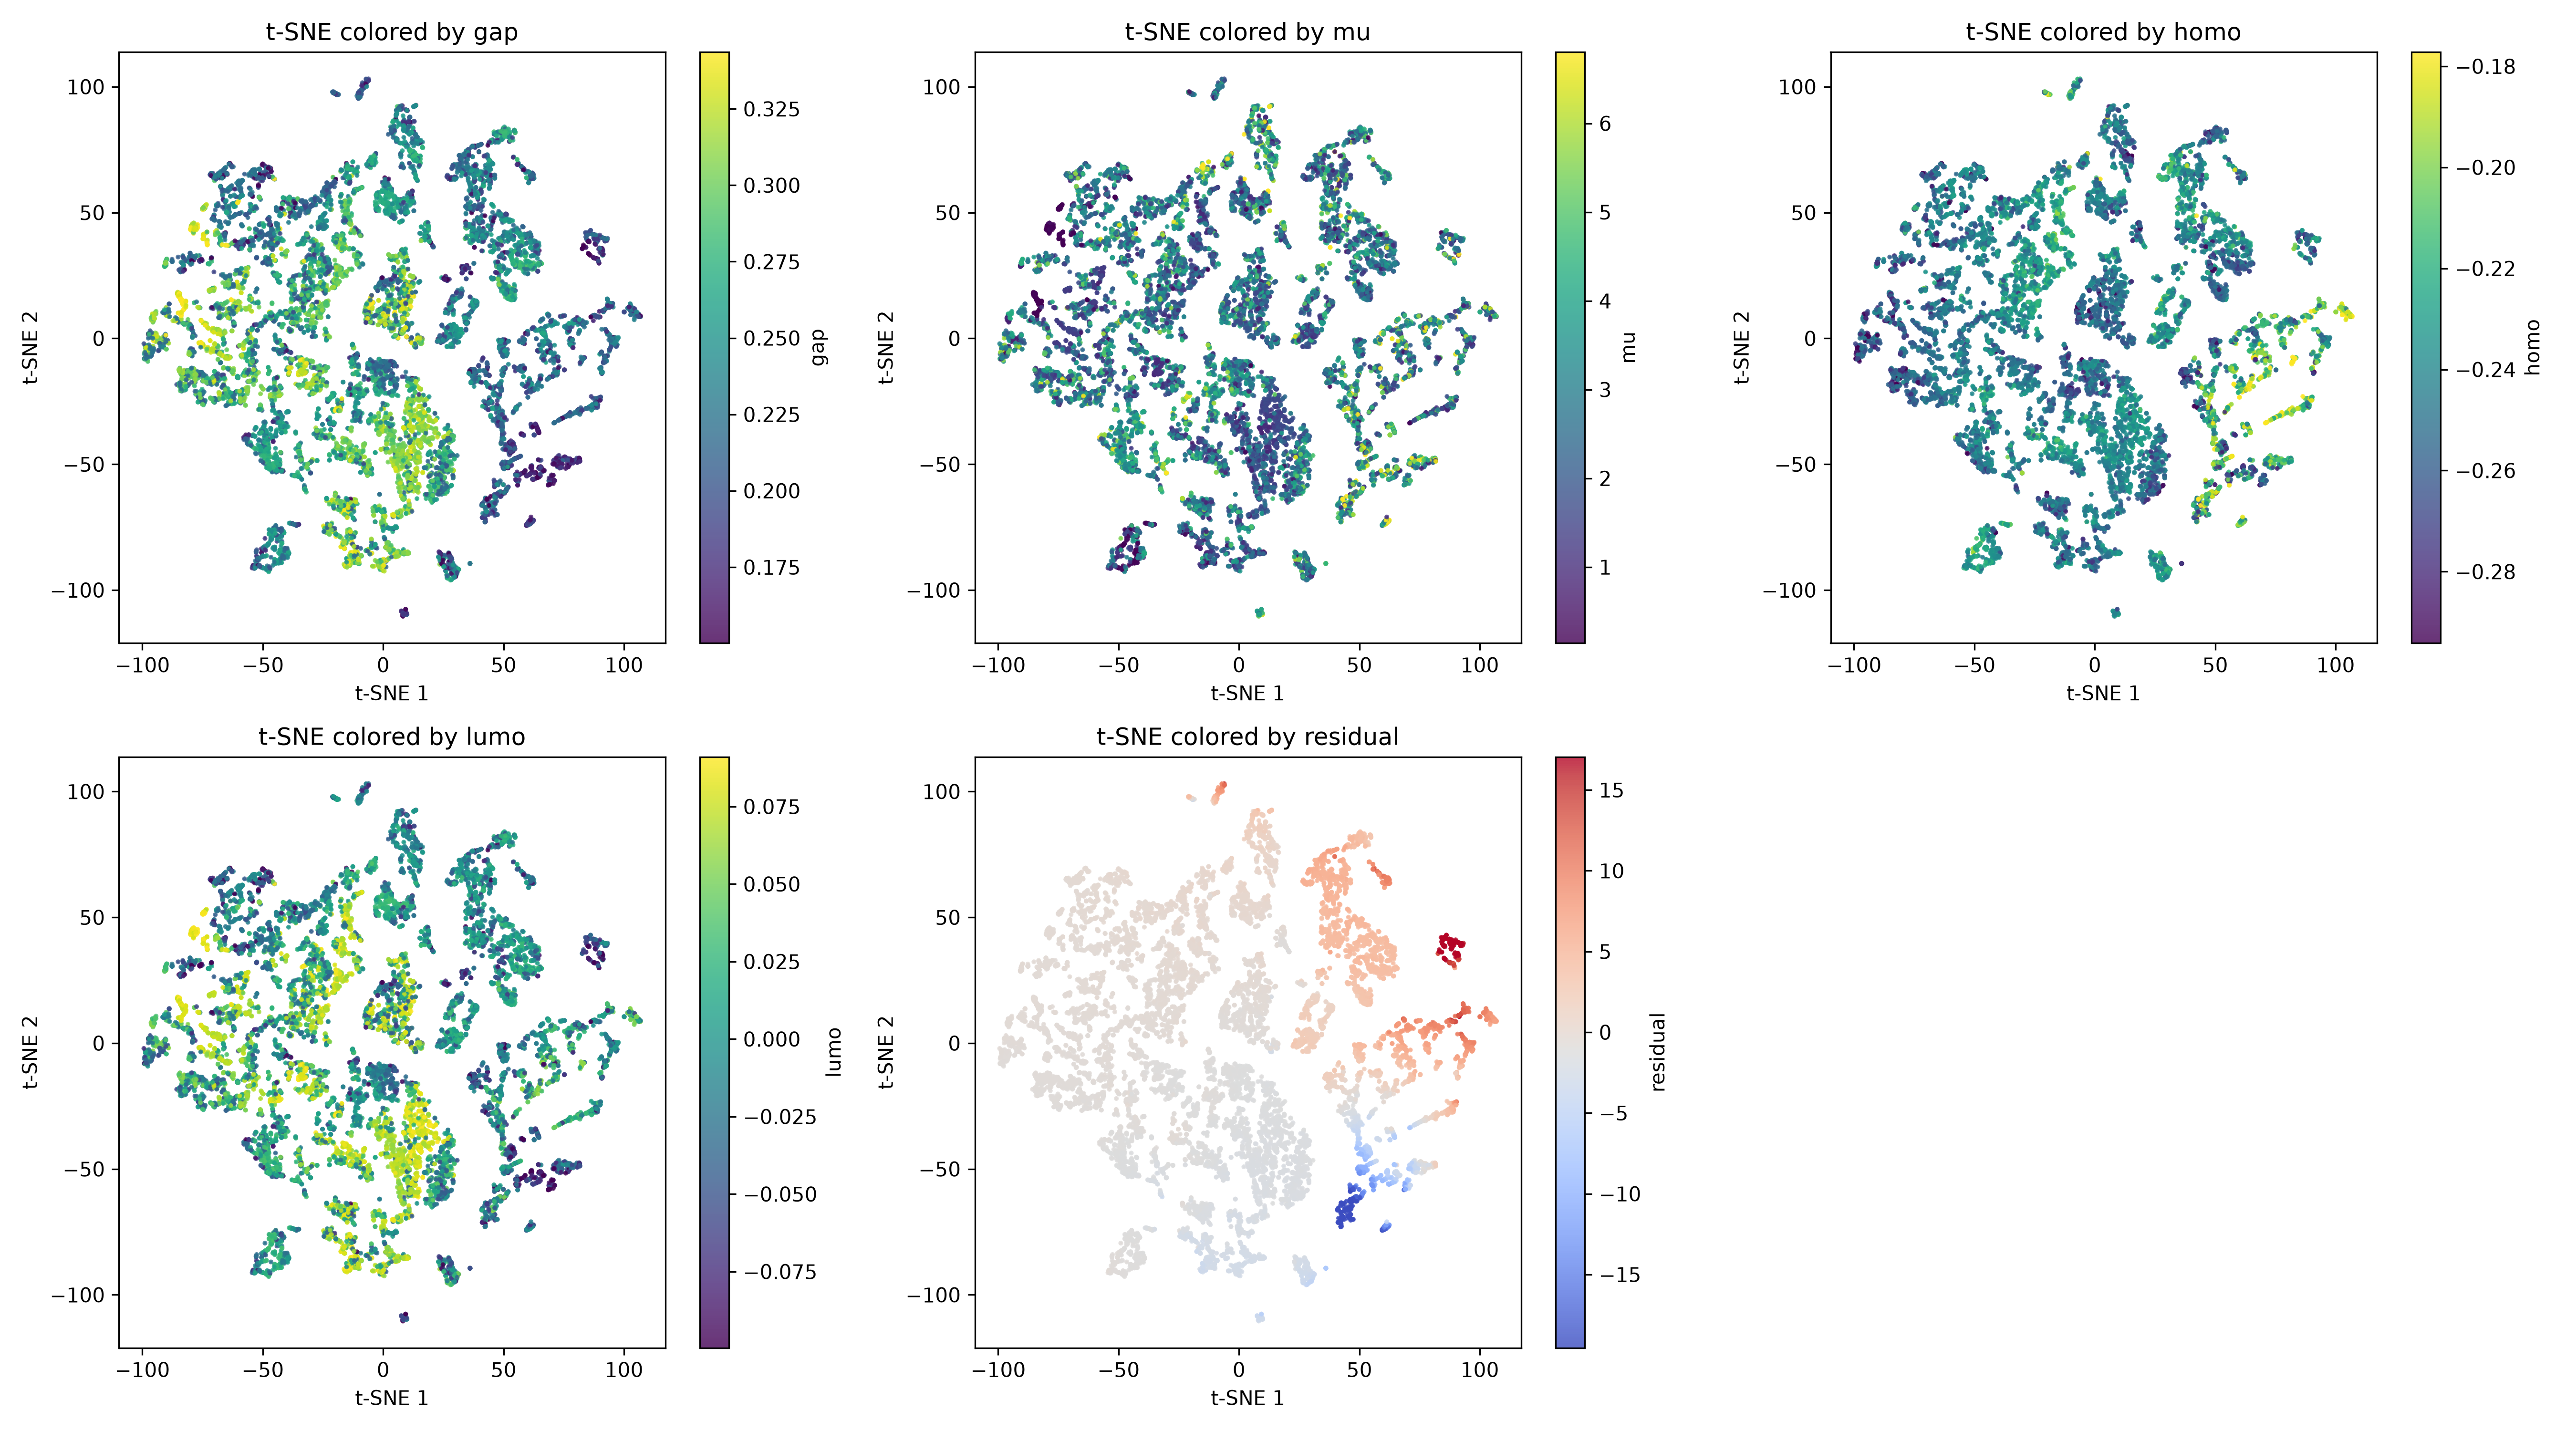
\includegraphics[width=0.99\textwidth]{../input_files/plots/tsne_property_scatter.png}    \caption{Two-dimensional t-SNE projection of the 128-dimensional latent space extracted from the trained Graph Neural Network (GNN). The scatter plots are colored by fundamental intensive electronic properties (HOMO-LUMO gap, dipole moment $\mu$, HOMO, and LUMO) alongside the target non-additive residual. The structured embedding landscape demonstrates that the network intrinsically learns underlying electronic structures without direct supervision. As visually captured, the first t-SNE dimension correlates with the HOMO-LUMO gap and HOMO energy, while the second dimension strongly orders the target non-additive residual. These distinct property gradients and clustering structures confirm that the GNN effectively models the non-linear electronic physics and non-additive energetics missed by classical additivity models.}    \label{fig:image2}\end{figure}\subsection{Structural motif attribution and statistical validation}To chemically interpret the non-additivity captured by the model, Integrated Gradients were applied to attribute energetic deviations to specific atomic and bond motifs  \citep{rao2021quantitativeevaluationexplainablegraph}. Molecules were partitioned based on the presence of identified high-influence topological features, specifically aromaticity, nitrogen, fluorine, and oxygen  \citep{lundstrom2022rigorousstudyintegratedgradients}. Statistical validation confirmed that these structural motifs are significant drivers of intensive electronic properties, as visualized in Figure \ref{fig:image3}.\begin{figure}[!tbp]    \centering    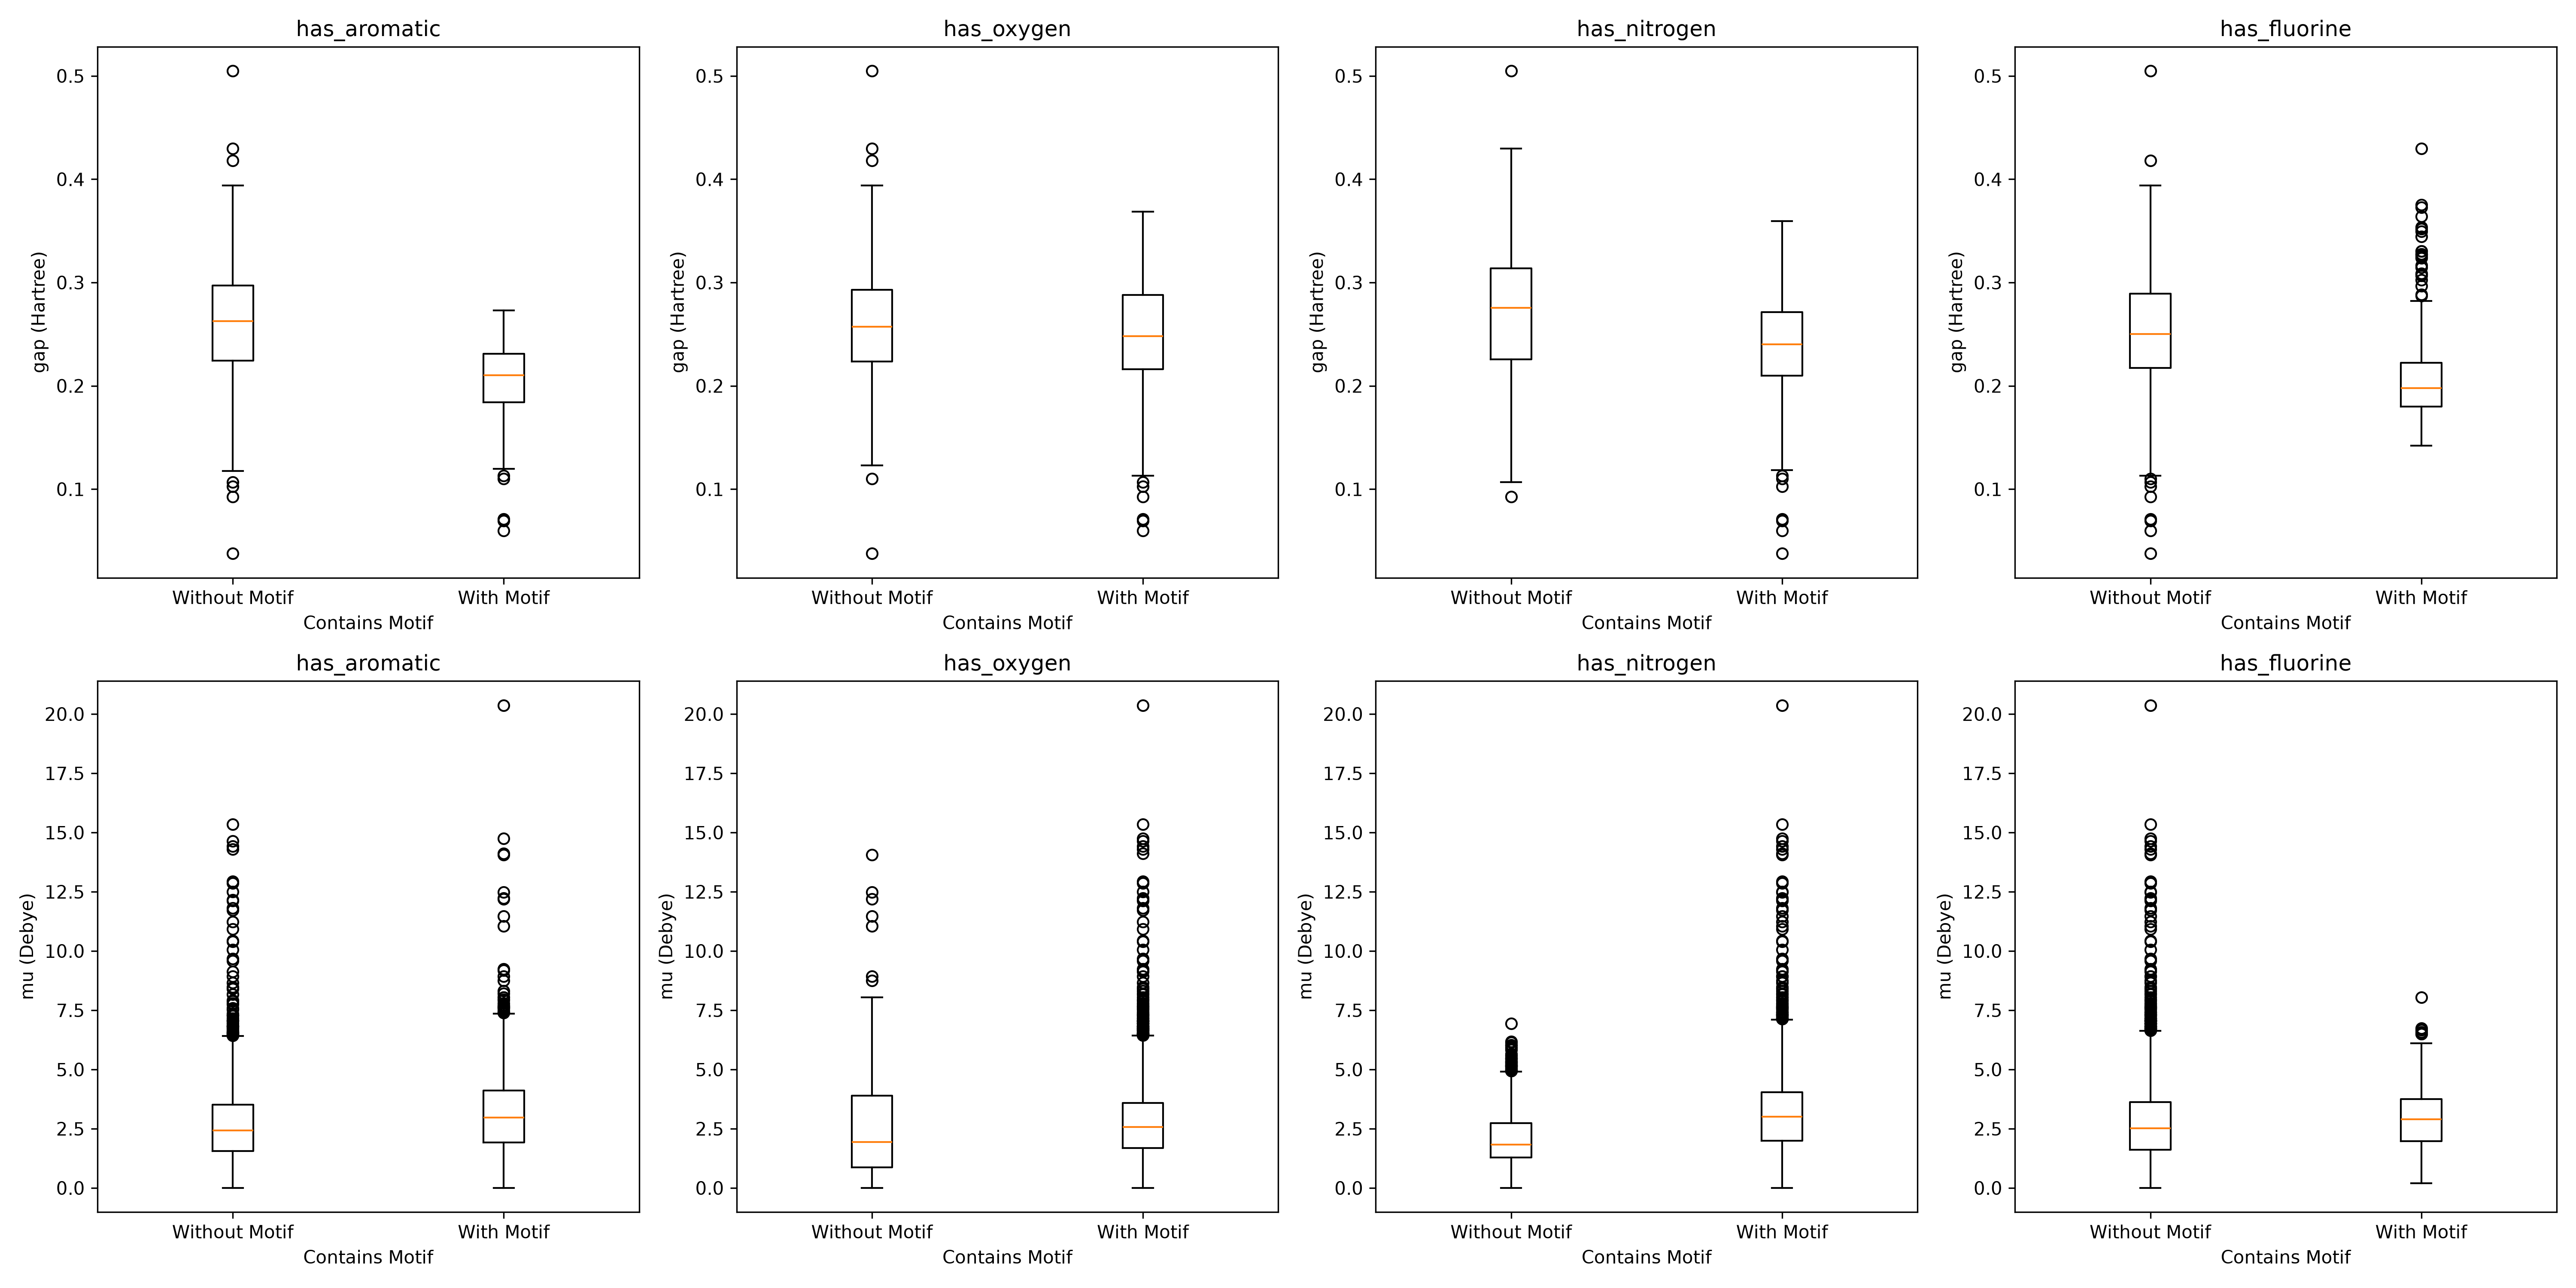
\includegraphics[width=0.99\textwidth]{../input_files/plots/motif_property_boxplots.png}    \caption{Boxplots illustrating the distributions of the HOMO-LUMO gap (top row, in Hartree) and dipole moment $\mu$ (bottom row, in Debye) for molecules partitioned by the presence of high-influence structural motifs: aromaticity, oxygen, nitrogen, and fluorine. The distributions reveal that the incorporation of these features—particularly aromatic rings and nitrogen—substantially compresses the HOMO-LUMO gap and increases the dipole moment. These statistically significant divergent distributions demonstrate that the energetic deviations from classical additivity, which are successfully captured by the Graph Neural Network, correspond directly to fundamental quantum-mechanical phenomena such as extended $\pi$-conjugation and heteroatom electronegativity.}    \label{fig:image3}\end{figure}Molecules containing aromatic motifs exhibit a significantly compressed HOMO-LUMO gap (mean $0.2071$ Hartree) compared to those without ($0.2608$ Hartree). A Kruskal-Wallis test confirms this difference is highly significant ($p < 0.0001$, Cohen's $d = -1.3990$). Furthermore, aromaticity significantly increases the dipole moment ($3.2036$ Debye vs. $2.6075$ Debye, $p < 0.0001$, Cohen's $d = 0.3734$). The integration of nitrogen similarly compresses the gap (mean $0.2396$ Hartree vs. $0.2704$ Hartree, $p < 0.0001$, Cohen's $d = -0.6734$) while massively shifting the dipole moment (mean $3.1419$ Debye vs. $2.0190$ Debye, $p < 0.0001$, Cohen's $d = 0.8312$). Fluorine incorporation also narrows the gap (mean $0.2133$ Hartree vs. $0.2519$ Hartree, ANOVA $p < 0.0001$, Cohen's $d = -0.7677$) and increases the dipole (mean $2.9627$ Debye vs. $2.7084$ Debye, ANOVA $p = 0.0162$, Cohen's $d = 0.1728$).Oxygen incorporation yields statistically significant but physically smaller shifts, modifying the gap (mean $0.2504$ Hartree vs. $0.2570$ Hartree, $p < 0.0001$, Cohen's $d = -0.1347$) and dipole (mean $2.7610$ Debye vs. $2.4275$ Debye, $p < 0.0001$, Cohen's $d = 0.2009$) . Further detailing the oxygen-containing groups, Figure \ref{fig:image1} highlights the specific distributions for motifs such as ethers and ketones, confirming that the incorporation of these topological features significantly shifts fundamental intensive electronic properties .\begin{figure}[!tbp]    \centering    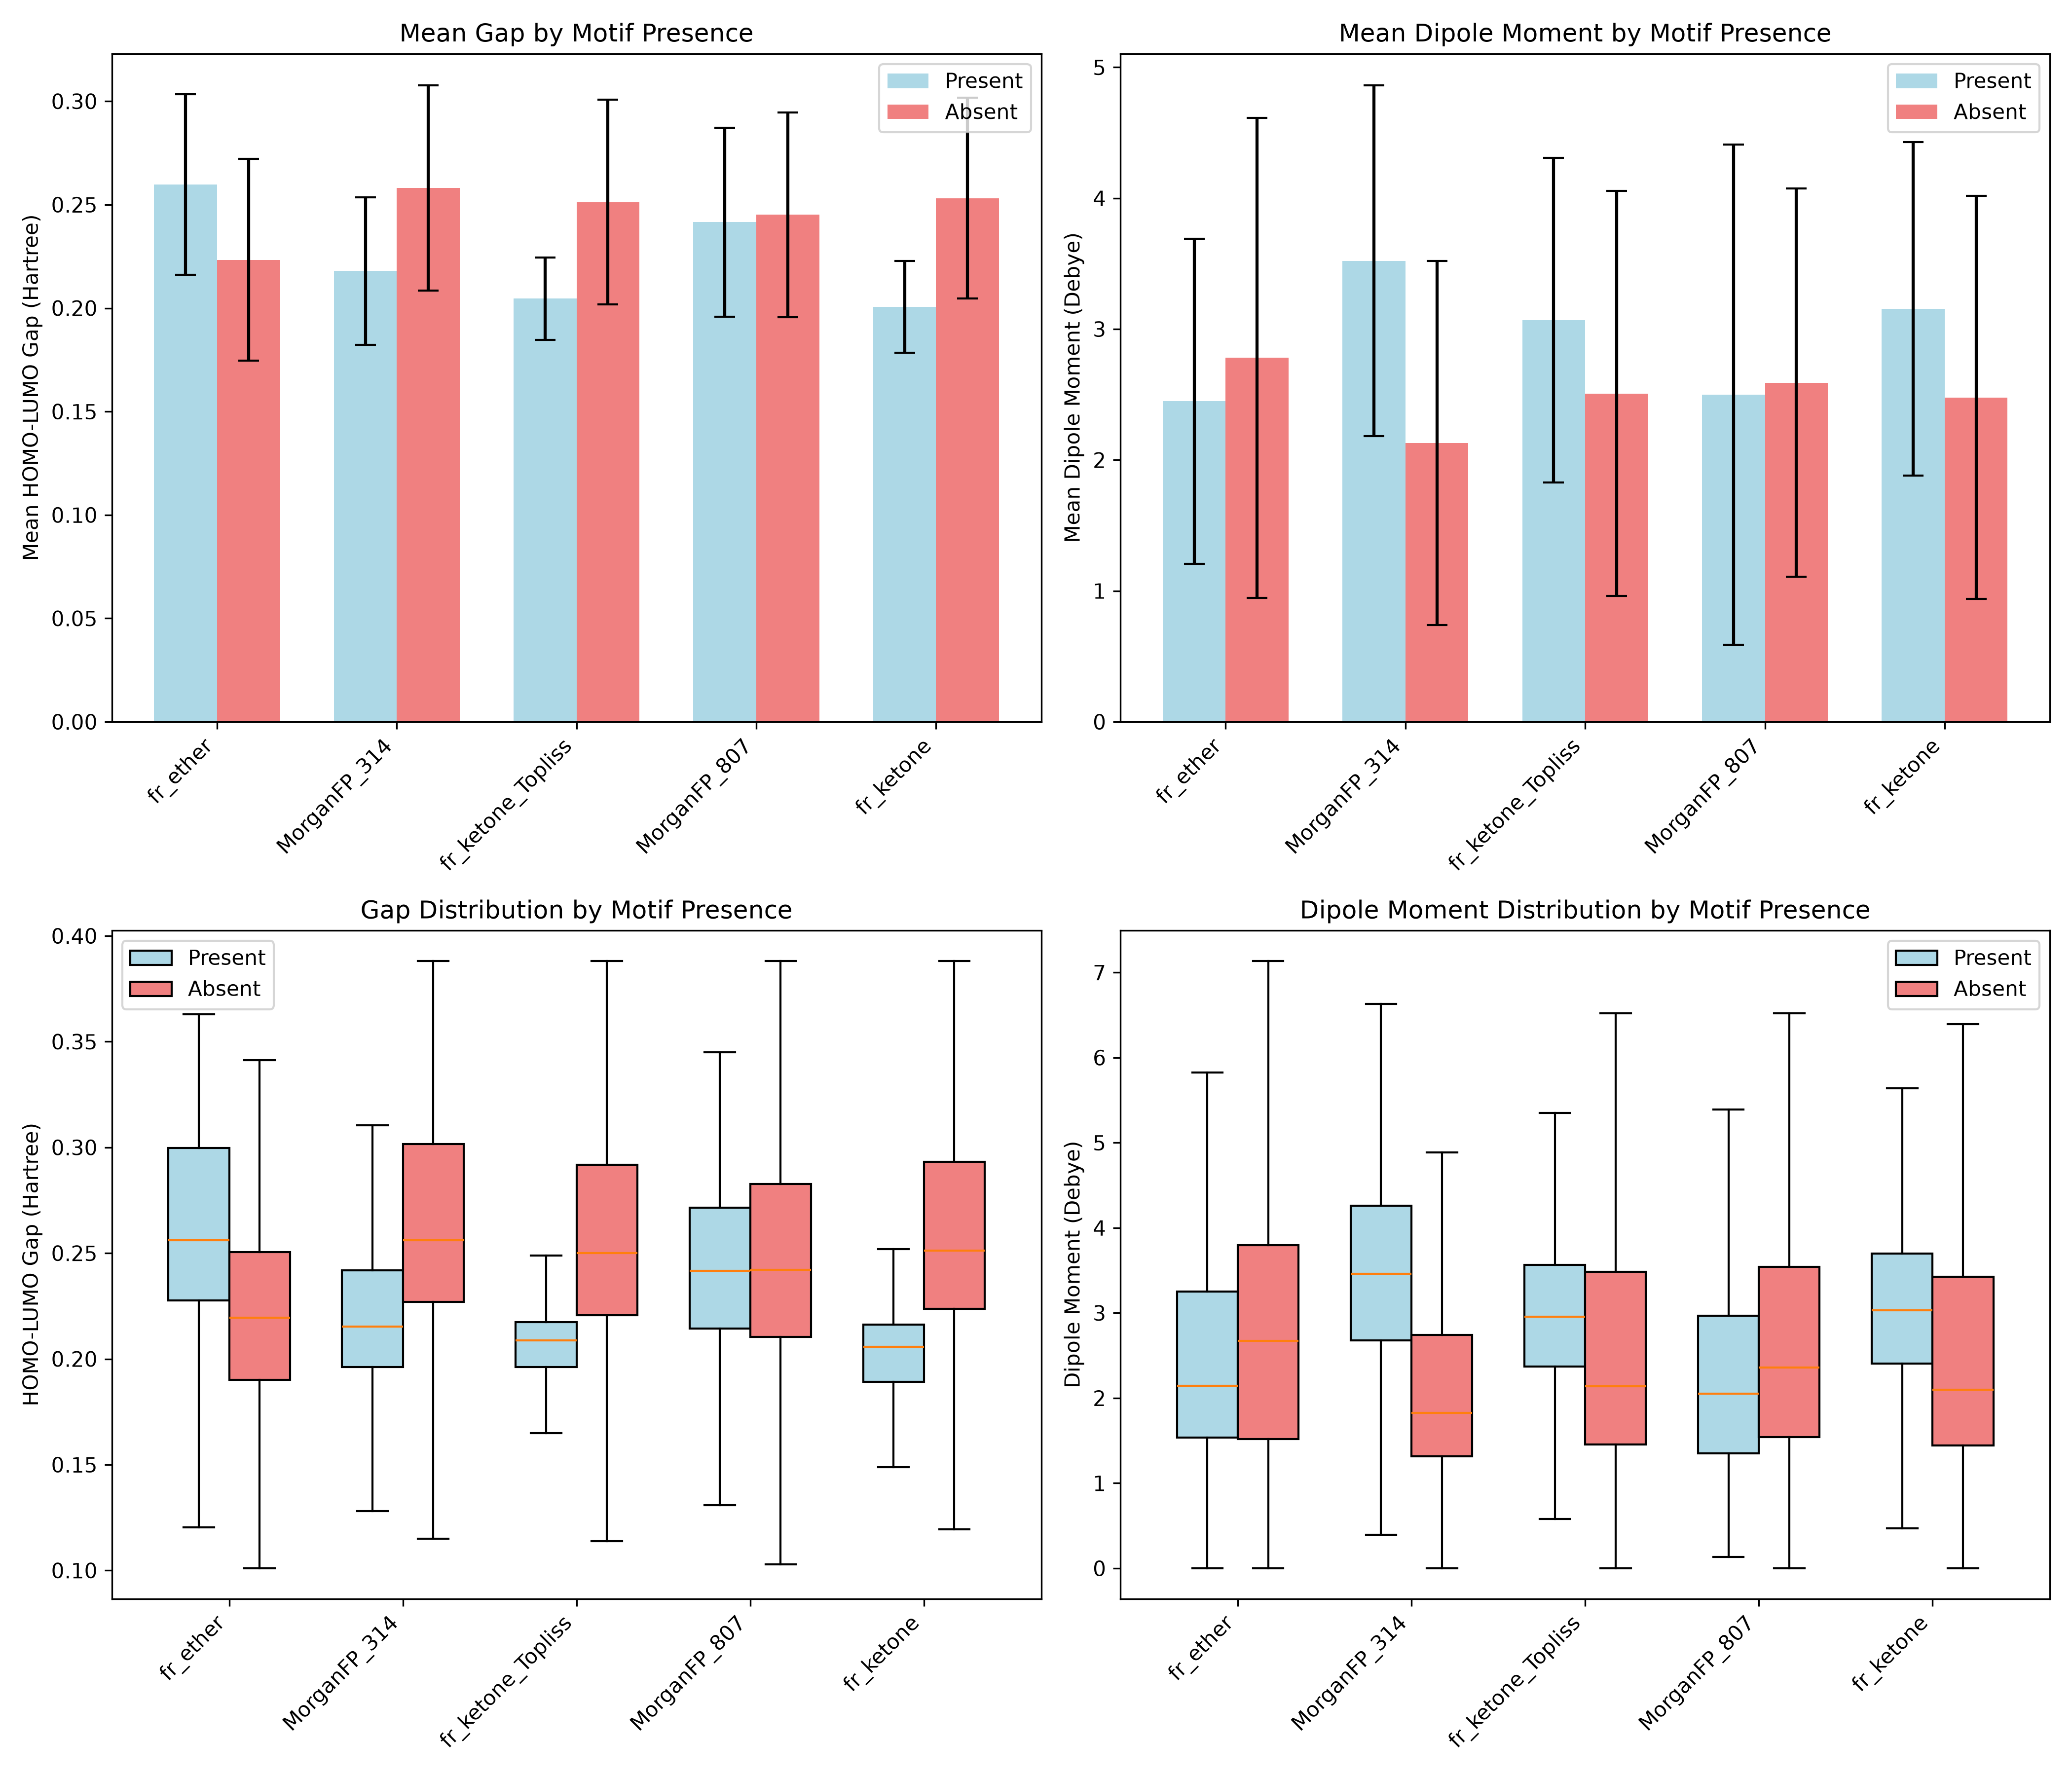
\includegraphics[width=0.99\textwidth]{../input_files/plots/motif_distributions.png}    \caption{Comparison of the HOMO-LUMO gap (left) and dipole moment (right) distributions based on the presence or absence of specific high-influence structural motifs, including oxygen-containing groups such as \texttt{fr\_ether} and \texttt{fr\_ketone}. The top panels display mean property values with error bars, while the bottom panels provide detailed boxplots of the divergent distributions. Consistent with statistical validation, the incorporation of these topological features significantly shifts fundamental intensive electronic properties. These structural attributions demonstrate that the graph neural network successfully learns underlying non-linear quantum-mechanical phenomena, effectively capturing the non-additive energetics that classical group-contribution baselines miss.}    \label{fig:image1}\end{figure}Overall, these divergent distributions demonstrate that the energetic deviations from classical additivity modeled by the GNN correspond directly to fundamental quantum-mechanical phenomena, such as extended $\pi$-conjugation and heteroatom electronegativity.

\section{Conclusions}
\label{sec:conclusions}
In this work, we introduced a graph-latent residual decomposition framework to rigorously isolate and quantify non-additive electronic effects from the extensive scaling inherent in molecular internal energy ($U_0$). By first establishing a classical group-contribution baseline using Ridge regression, we successfully decoupled size-dependent energetic scaling. The remaining residuals, representing purely non-linear quantum-mechanical deviations, were then modeled using a Graph Neural Network (GNN). Our results demonstrate that explicit graph-based message passing is highly effective at capturing these topological nuances. The GNN achieved a test $R^2$ of 0.9985 on the standardized residuals, substantially outperforming a descriptor-based Random Forest baseline and confirming that molecular topology is essential for modeling complex electronic physics.Beyond predictive accuracy, this framework provides deep interpretability into the learned representations of non-additivity. Analysis of the GNN's 128-dimensional latent space revealed that the network intrinsically learned to encode fundamental intensive properties, such as the HOMO-LUMO gap and HOMO energy, despite receiving no direct supervision on these targets. Dimensionality reduction further illustrated a highly structured embedding landscape where distinct property gradients align with the modeled energetic deviations, proving that the network captures genuine quantum-mechanical phenomena rather than arbitrary statistical variance.Furthermore, by applying Integrated Gradients, we successfully mapped these non-additive energetic deviations back to specific structural motifs \citep{sundararajan2017axiomaticattributiondeepnetworks,polat2025xchemagentsagenticaiexplainable,ji2026molledgeradditivegraphneural}. Statistical validation confirmed that features such as aromatic rings and the integration of highly electronegative heteroatoms (nitrogen and fluorine) are significant drivers of non-additivity \citep{lundstrom2022rigorousstudyintegratedgradients,wang2026explainablemolecularpropertyprediction}. These motifs correspond directly to physically observable shifts, notably compressed HOMO-LUMO gaps and increased dipole moments, which are characteristic of extended $\pi$-conjugation and complex electron localization \citep{chen2026interpretablemachinelearningquantuminformed,mick2026datafusioncontrastivealignment,bigting2026martinimapperautomatedfragmentbased}.Ultimately, this approach bridges the gap between classical additivity models and advanced deep learning techniques. By explicitly separating extensive scaling from underlying non-linear electronic physics, our framework not only improves predictive performance but also provides a chemically intuitive mapping of how specific structural motifs deviate from classical group-contribution theory. This methodology offers a robust and interpretable tool for future computational chemistry applications, enabling more targeted molecular design and a deeper understanding of structure-property relationships without the computational overhead of 3D coordinate generation.


\bibliography{bibliography}{}
\bibliographystyle{unsrt}

\end{document}
